\documentclass[conference]{IEEEtran}
\IEEEoverridecommandlockouts
% The preceding line is only needed to identify funding in the first footnote. If that is unneeded, please comment it out.
\usepackage{cite}
\usepackage{amsmath,amssymb,amsfonts}
\usepackage{algorithmic}
\usepackage{graphicx}
\usepackage{textcomp}
\usepackage{xcolor}
\usepackage{multirow}
\usepackage{pgfplots}
\def\BibTeX{{\rm B\kern-.05em{\sc i\kern-.025em b}\kern-.08em
    T\kern-.1667em\lower.7ex\hbox{E}\kern-.125emX}}
\begin{document}

\title{Recommender Systems}

\author{\IEEEauthorblockN{mbkb74}
    \IEEEauthorblockA{\textit{Department of Computer Science} \\
        \textit{Durham University}\\
        Durham, United Kingdom \\}

}

\maketitle

\begin{abstract}
    This paper implements a hybrid recommender system on the Yelp dataset. It uses collaborative and content-based filtering with a weighted scheme.
\end{abstract}

\begin{IEEEkeywords}
    Recommender systems, collaborative filtering, content filtering, hybrid filtering
\end{IEEEkeywords}

\section{Introduction}

\subsection{Domain of application}

This application works on Italian restaurants.

\subsection{Related work review}

There are a wide range of papers on recommender systems, in this paper I will be comparing my recommender system to one on a movie dataset \cite{evaluation} and one on big data in education \cite{dwivedi2017recommender} as the authors have applied a range of evaluation techniques that allows me to compare my produce recommender to theirs.

\subsection{Purpose/aim}

The aim of this application is to recommend an Italian restaurant to the user.


\section{Methods}

\subsection{Data description}

The data is from the Yelp dataset \cite{b1}, this contains a list of the businesses on Yelp, detailing which categories they fall under. It also contains all the reviews, including a written review along with a range of scores. This also now contains a COVID-19 dataset, which lists the changes businesses are making due to COVID-19. There are around 8 million reviews in the review dataset.

\subsection{Data preparation and feature selection}

In order to make the data easier to process, along with increasing the accuracy of predictions, it is needed to reduce the number of reviews. First I selected just restaurants, but as this is a large part of Yelp, it only reduced the dataset to 5 million reviews. So I have reduced it to just Italian restaurants, shrinking the dataset to around 470k reviews. In addition, limiting the timescale reduces the impact of tastes changing over time, so I have only included reviews after 2016. This reduced the number of reviews to around 270k, which is enough to give a good sample, but small enough to be practical to process.

\subsection{Hybrid scheme}

This uses a weighted hybrid scheme, with each recommender contributing half towards the final result. The scores for each are summed and halved to generate a final score for each restaurant.

\subsection{Recommendation techniques/algorithms}

There are two recommenders used here, content-based filtering and collaborative filtering. The content-based filtering works on the text of the reviews to find reviews that use similar words. An example of this is that if someone describes a restaurant as "cosy", then it will find other reviews that use the same word. Collaborative filtering looks at the restaurants the user has reviewed and finds people who have reviewed those restaurants in the same way and looks at their reviews of other restaurants to find the best restaurants.

Furthermore the COVID-19 dataset is used to check the list of suggested restaurants and remove those that are closed as the user wouldn't be able to visit them.

\subsection{Evaluation methods}

Usage predictions are generated by removing half of the user's reviews, and predicting which restaurants they would like, and seeing how many of the hidden reviews are recommended to the user. These statistics are generated by mapping the ratings and user scores onto either 0 or 1, with 0 being that they don't like it and 1 being that they do. This allows for the generation of a confusion matrix, which is then used to produce the metrics.

Rating predictions use a very similar methodology to usage predictions, but instead of mapping to 0 or 1, map the results so they are in the range [0,1], then perform the root mean square error on them. 

Coverage metrics are calculated by listing the number of businesses before and after the users are removed, and dividing the two gives the prediction coverage value.


\section{Implementation}

\subsection{Input interface}

For the input to this application, the user can choose which user they are from a list of 10 randomly selected users from a list of users that have made lots of reviews. This is done so that the recommenders have more data to work with, providing more accurate results.

\subsection{Recommendation algorithm}

I find the count of the reviews for each business, and for each user I find how many reviews they have left. Then I only select the 300 most reviewed businesses, this allows for better predictions to be made. I then choose the 100 users who have left the most reviews and take a random sample of 10 to present to the user of the program. Likewise this allows for better predictions. Obviously in a real application you would choose your user from the whole set of users, but this provides more interesting data.

This is where I use content based filtering. From \texttt{sklearn} I use the \texttt{TfidfVectorisor} to get the TF-IDF matrix, then use the \texttt{linear\_kernel} function between this matrix and the same matrix, but only including the user reviews. I then use these scores and choose the 300 best matches and merge this with the 300 most reviewed businesses previously found, to generate a smaller list where the restaurant is in both sets.

For each users rating of a restaurant, I group repeated ratings of the same restaurant as the average, this allows for better representation as one person rating the same restaurant 5 stars lots of time shouldn't have more impact than once. I then generate the cosine similarity between all the restaurants as a matrix, using the ratings. For each restaurant the recommender wants to get a prediction for, the recommender loops over the cosine similarities generated for that item. This is to generate an adjusted weighted average.

This concludes the collaborative filtering section. I then choose the 5 largest scores to present to the user, and remove any which are shown in the COVID dataset as not open.

\subsection{Output interface}

The output for this system is a list of 5 restaurants the user would most like, along with their COVID-19 notice so the user knows how to prepare. This also displays a percentage to the user which is the weighted average calculated by the hybrid recommender to be more transparent about why they are being recommended and so that they can better compare the restaurants.

\section{Evaluation results}

\subsection{Comparison against baseline implementation}

\subsubsection{Usage Metrics}


\begin{flushleft}
	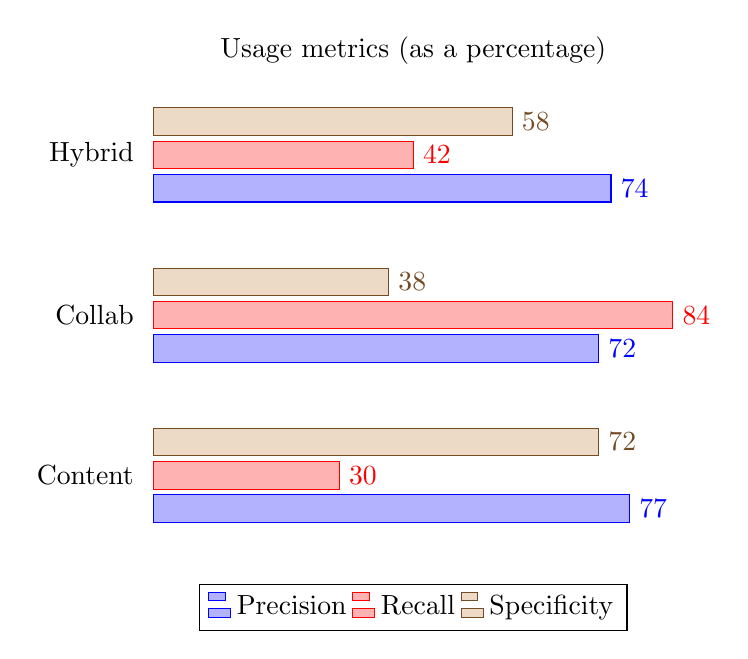
\begin{tikzpicture}
		\begin{axis}[title  = Usage metrics (as a percentage),
			xbar,
			y axis line style = { opacity = 0 },
			axis x line       = none,
			tickwidth         = 0pt,
			ytick             = data,
			enlarge y limits  = 0.2,
			enlarge x limits  = 0.02,
			xmin=0,
			nodes near coords,
          	legend style={at={(0.5,-0.1)},
				anchor=north,legend columns=-1},
			symbolic y coords = {Content, Collab, Hybrid},
			]
			\addplot coordinates { (72,Collab) (77,Content)
				(74,Hybrid)   };
			        \addplot 
			coordinates {(84,Collab) (30,Content) 
				(42,Hybrid) };
			\addplot 
			coordinates {(38,Collab) (72,Content) 
				(58,Hybrid) };
			\legend{Precision,Recall,Specificity}
		\end{axis}
	\end{tikzpicture}
\end{flushleft}


Collaborative filtering has poor specificity, not predicting negative values well, whereas content-based filtering has poor recall, not predicting positive values well. This is a good case for a hybrid recommender as my merging them it helps to smooth the incorrect results.

\subsubsection{Coverage}

As part of the filtering of the data, I remove all users who have just reviewed one restaurant as it prevents comparison. This reduces the total number of restaurants from 3120 to 2469, giving a prediction coverage of 79\%. This is the same for my baseline and hybrid implementations.

\subsection{Rating}

For the rating metric I used root mean square error, which gave the following results
\begin{itemize}
	\item Hybrid: 0.345
	\item Collaborative: 0.357
	\item Content-Based: 0.371
\end{itemize}

This shows that by combining the results from collaborative and content-based filtering, I get a recommender that outperforms them both. Also all of these values are reasonably low, showing that the recommenders are all fairly good.


\subsection{Comparison against hybrid recommenders in related studies}

\subsubsection{Usage Metrics}

In \cite{evaluation}, they implement the same recommenders, but on a movie dataset. The content based recommender has precision of 0.68 and recall of 0.42. My recommender has a higher precision, but lower recall. The collaborative recommender had precision of 0.69 and recall of 0.84. For this I got a higher score in both statistics. Their final hybrid recommender has precision of 0.8 and recall of 0.45, my results for both of these are slightly lower, but not by a significant margin.

\subsubsection{Coverage}

In \cite{evaluation}, they filter user profiles that have over 100 rated items, reducing the number of profiles from 61265 to 7164, giving prediction coverage of 12\%. Similarly to my recommender, this value is the same for baseline and hybrid.

\subsubsection{Rating}

Unfortunately the source given for the previous two metrics didn't calculate a rating prediction, however a different recommender for education calculated a root mean square error of 0.46, which is worse than the 0.345 best for my hybrid recommender \cite{dwivedi2017recommender}.

\subsection{Ethical Issues}

The data has been anonymised to some degree as reviews just include the \texttt{userid}, however using the yelp website, this then takes you to the person's profile. From there it's up to the user how anonymous they make their profile, but they are fairly good in that they don't show other social links to find out more about users.

All the data in the dataset is explicit in that the user has submitted this to the website, rather than it being inferred from their behaviour.

The algorithm is provided to the user so they can see what it does, and it shouldn't have any bias other than that provided to it in the form of the reviews submitted.

This has the potential to influence people's behaviour by encouraging them to go to certain restaurants. However manipulating people into going to certain restaurants is unlikely to cause a lasting change on their behaviour outside of that instance.



\section{Conclusion}

This recommender is limited by the data provided to it. People don't leave lots of reviews, and so this limits the capabilities of both recommenders in their functionality. Also, I want this to run in a reasonable amount of time, so the set of reviews has been filtered down to a small timescale and category, it is likely that the predictions would be better if they had more data.


\bibliographystyle{IEEEtran}
\bibliography{report}



\end{document}
